%\documentclass{article}
%\usepackage{graphicx,subfigure,lscape}

%\newcommand{\goodgap}{%
%  \hspace{\subfigtopskip}%
%  \hspace{\subfigbottomskip}}

%\begin{document}

%\begin{landscape}
\begin{figure}[p]
  \centering
  \subfigure[Plate (i) x... magnification.]{
    \label{fig:9(i)}
    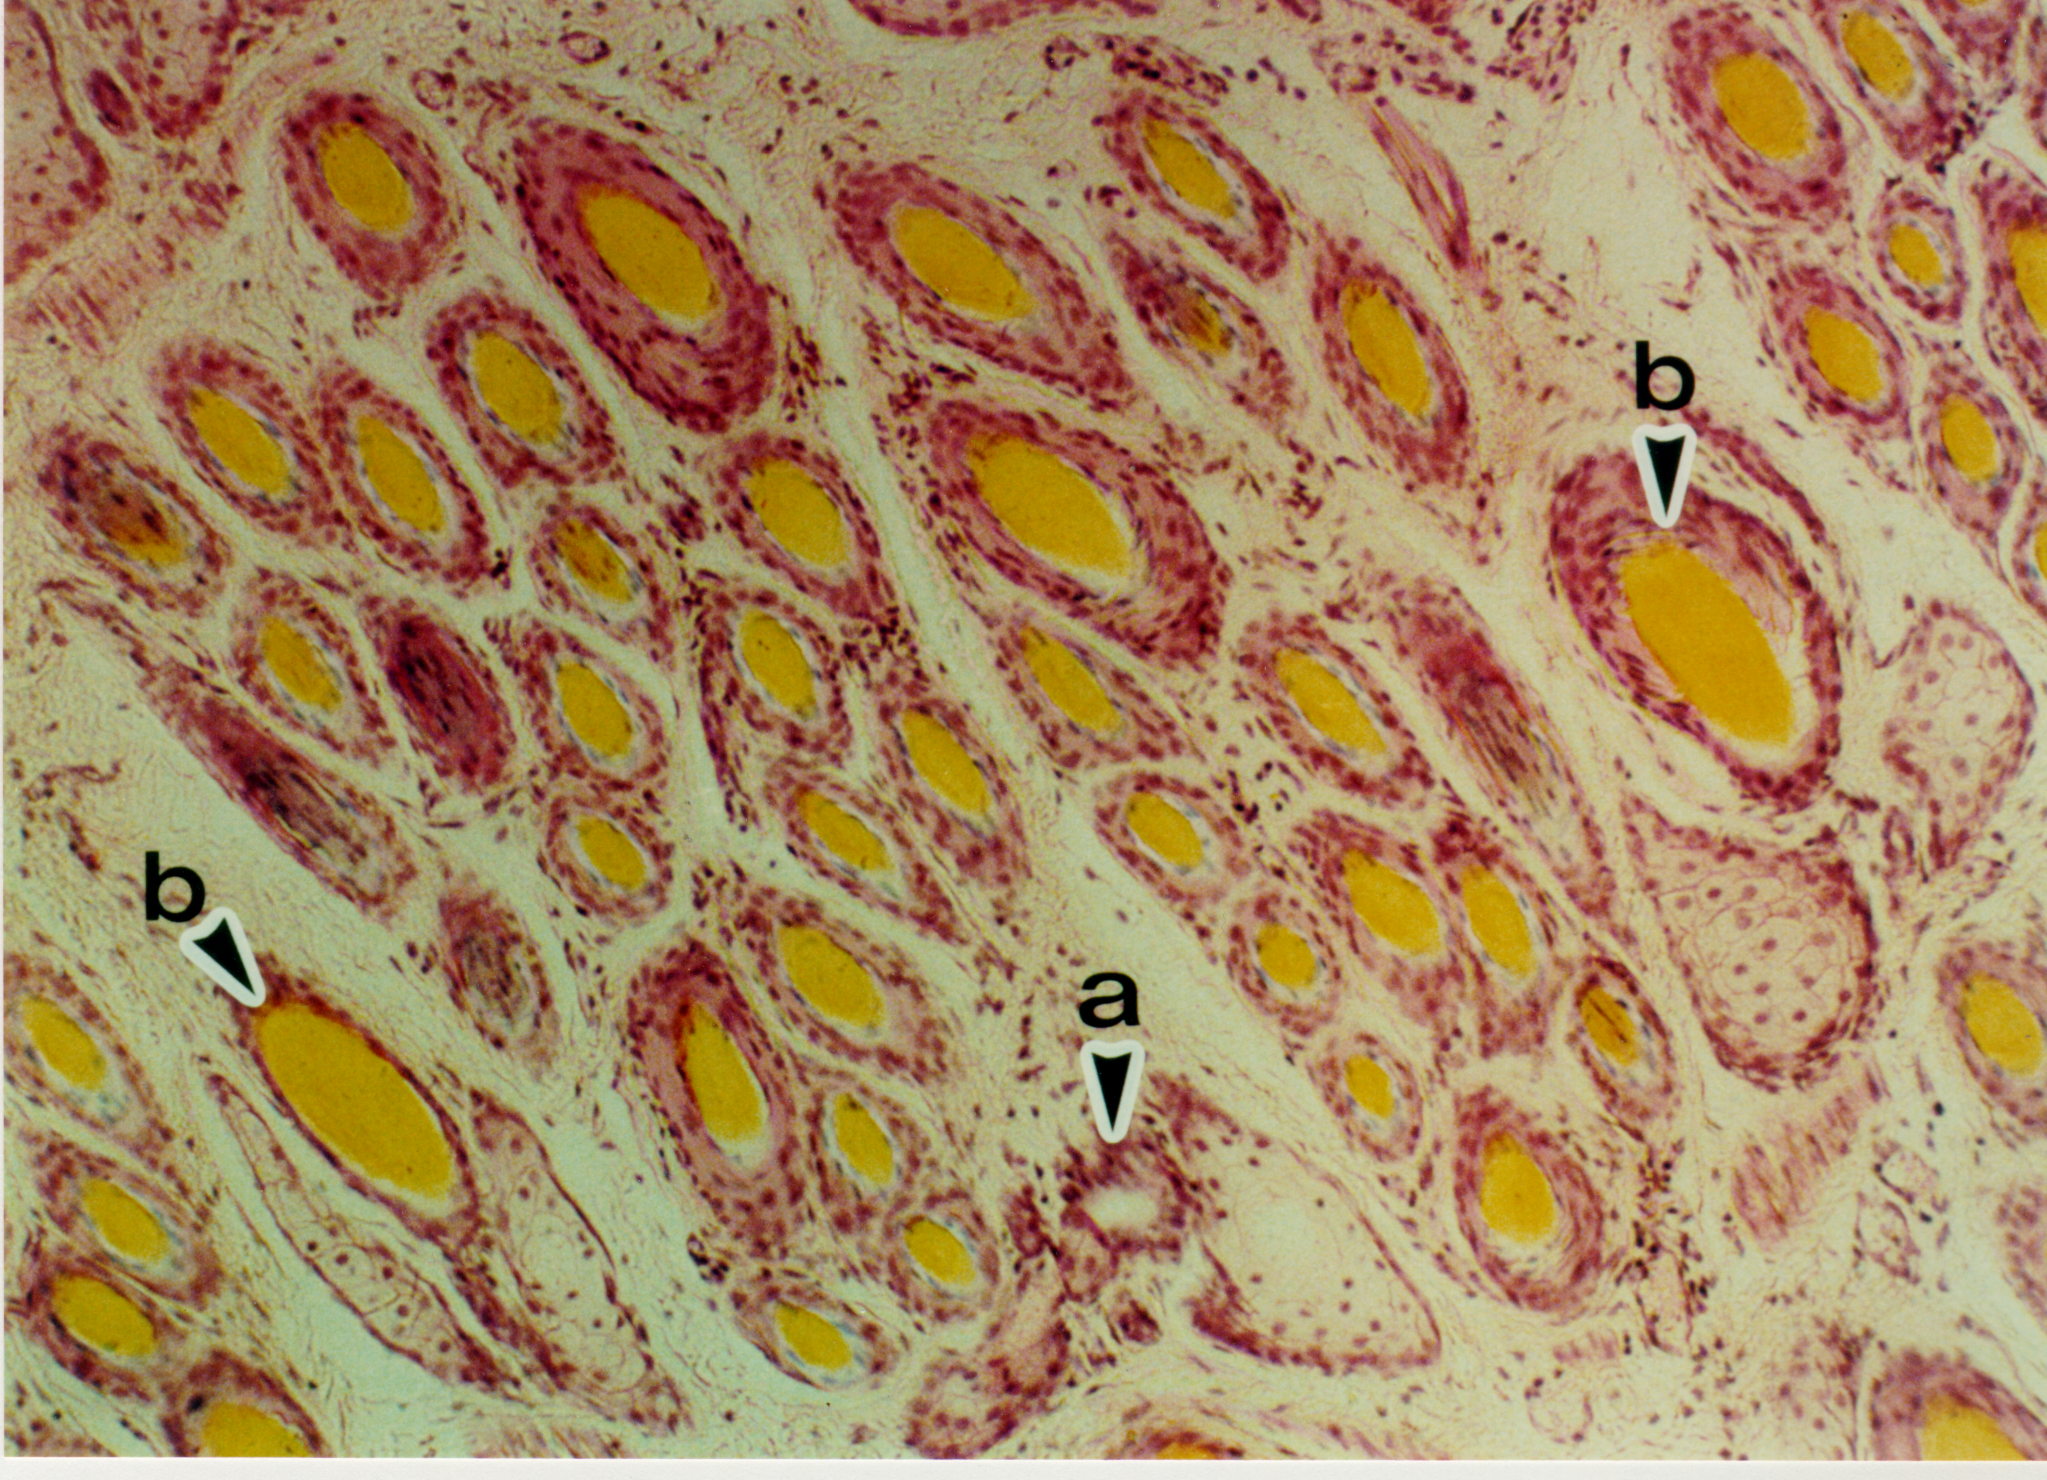
\includegraphics[width=0.65\textwidth, trim = 0 20 0 140]{images/fig9a.png}
  }
  \subfigure[Plate (ii) x... magnification.]{
    \label{fig:9(ii)}
    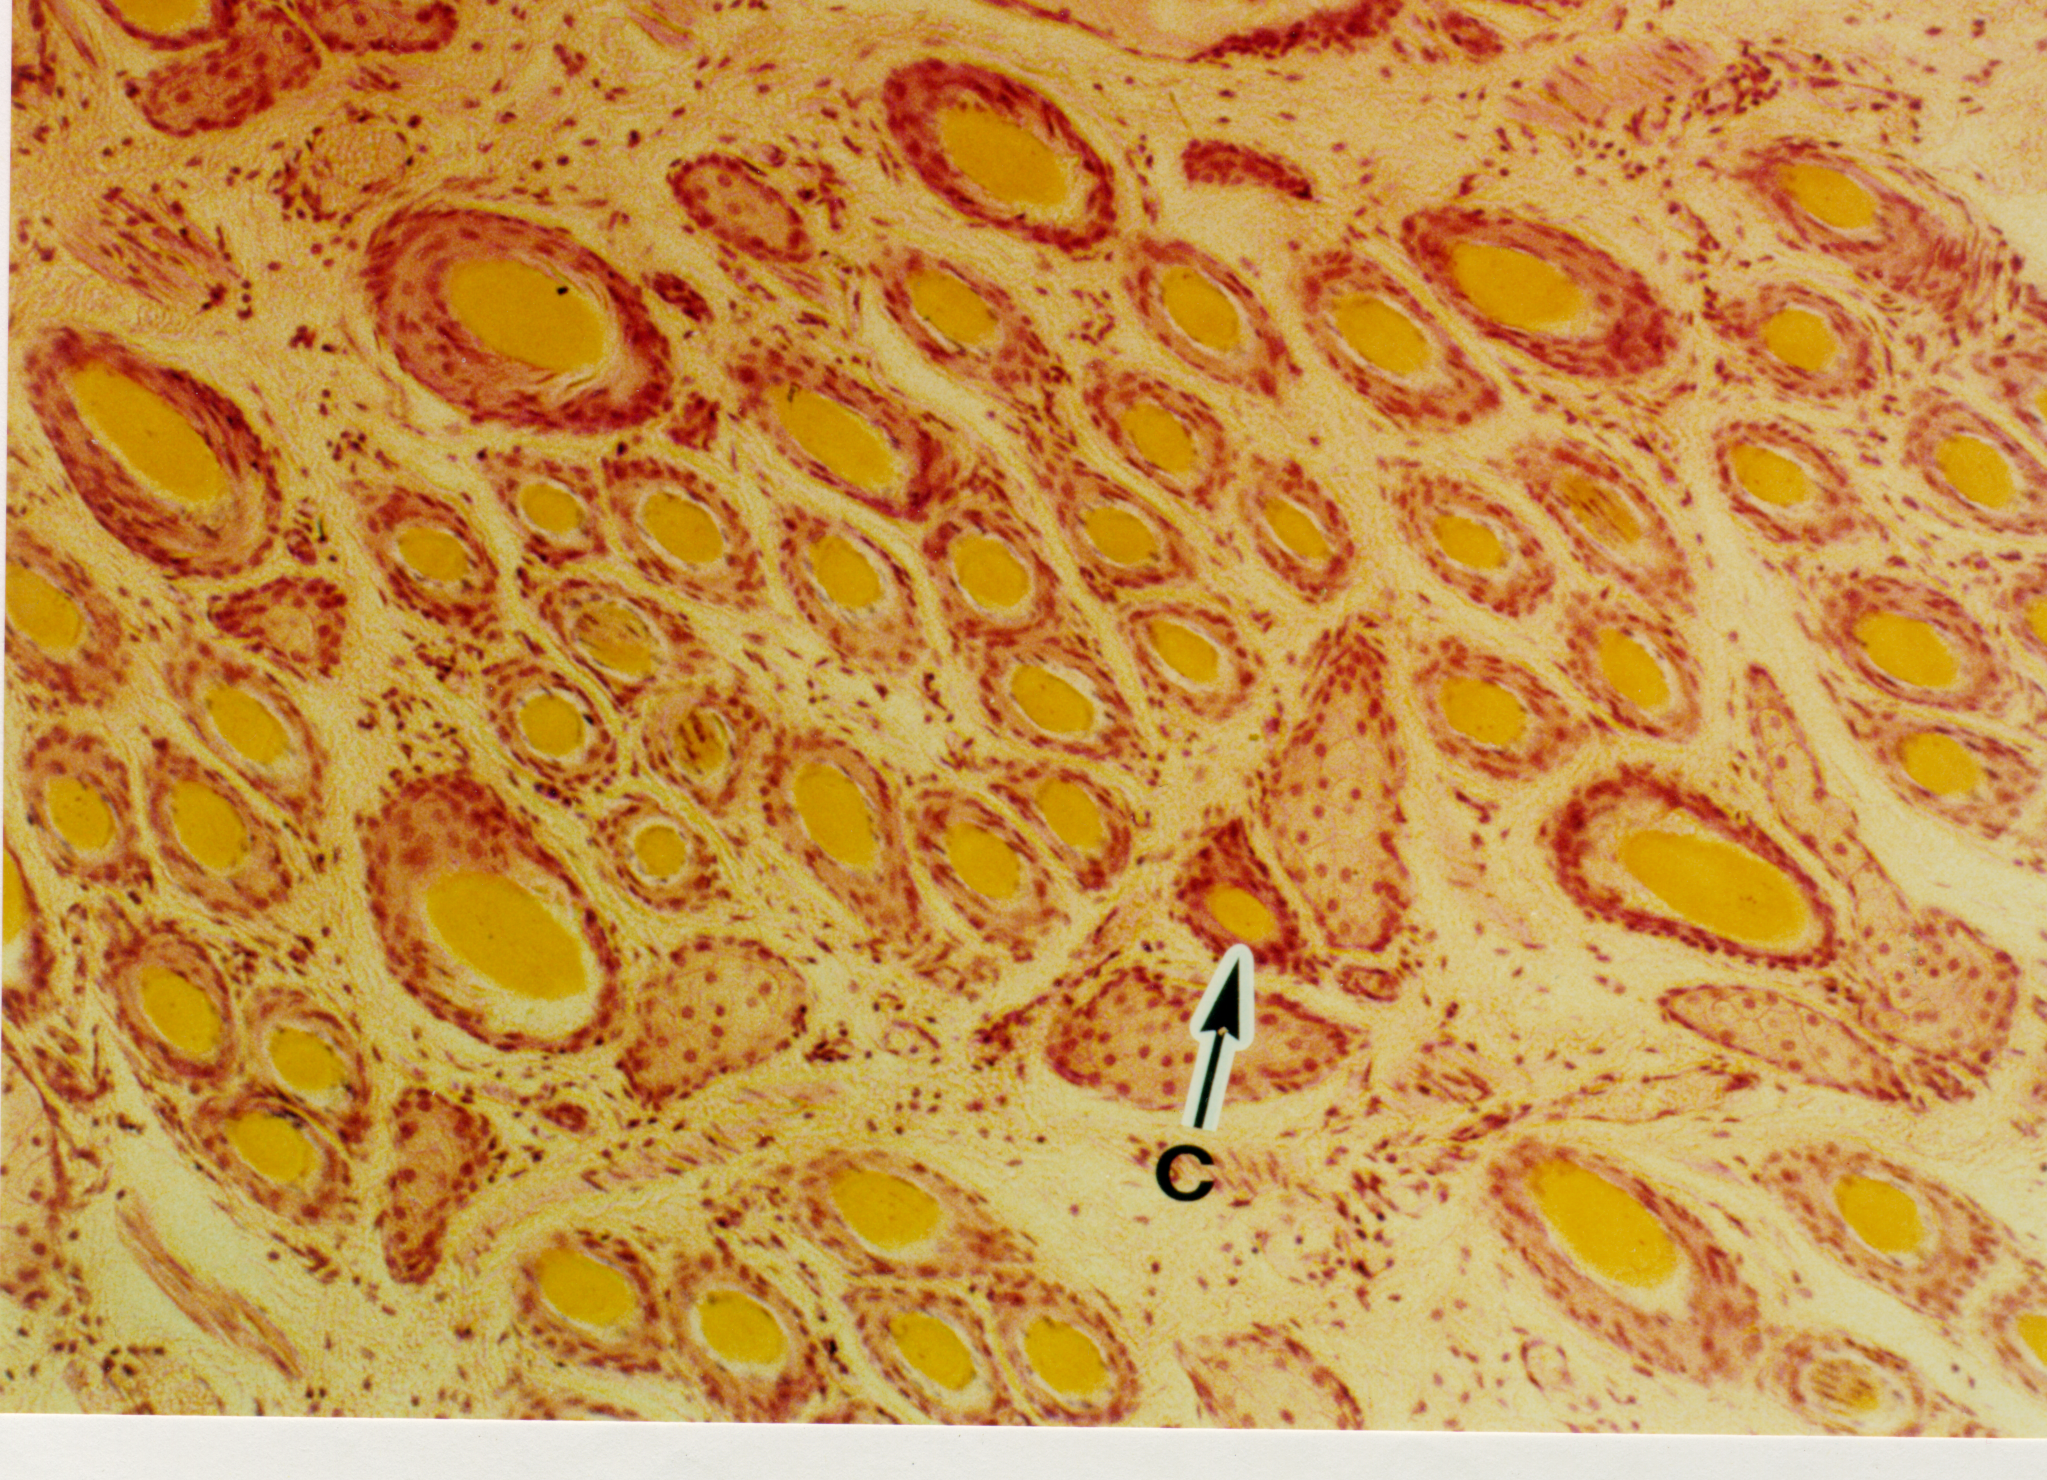
\includegraphics[width=0.65\textwidth, trim = 0 20 0 20]{images/fig9b.png}
  }
  \subfigure[Plate (iii) x... magnification.]{
    \label{fig:9(iii)}
    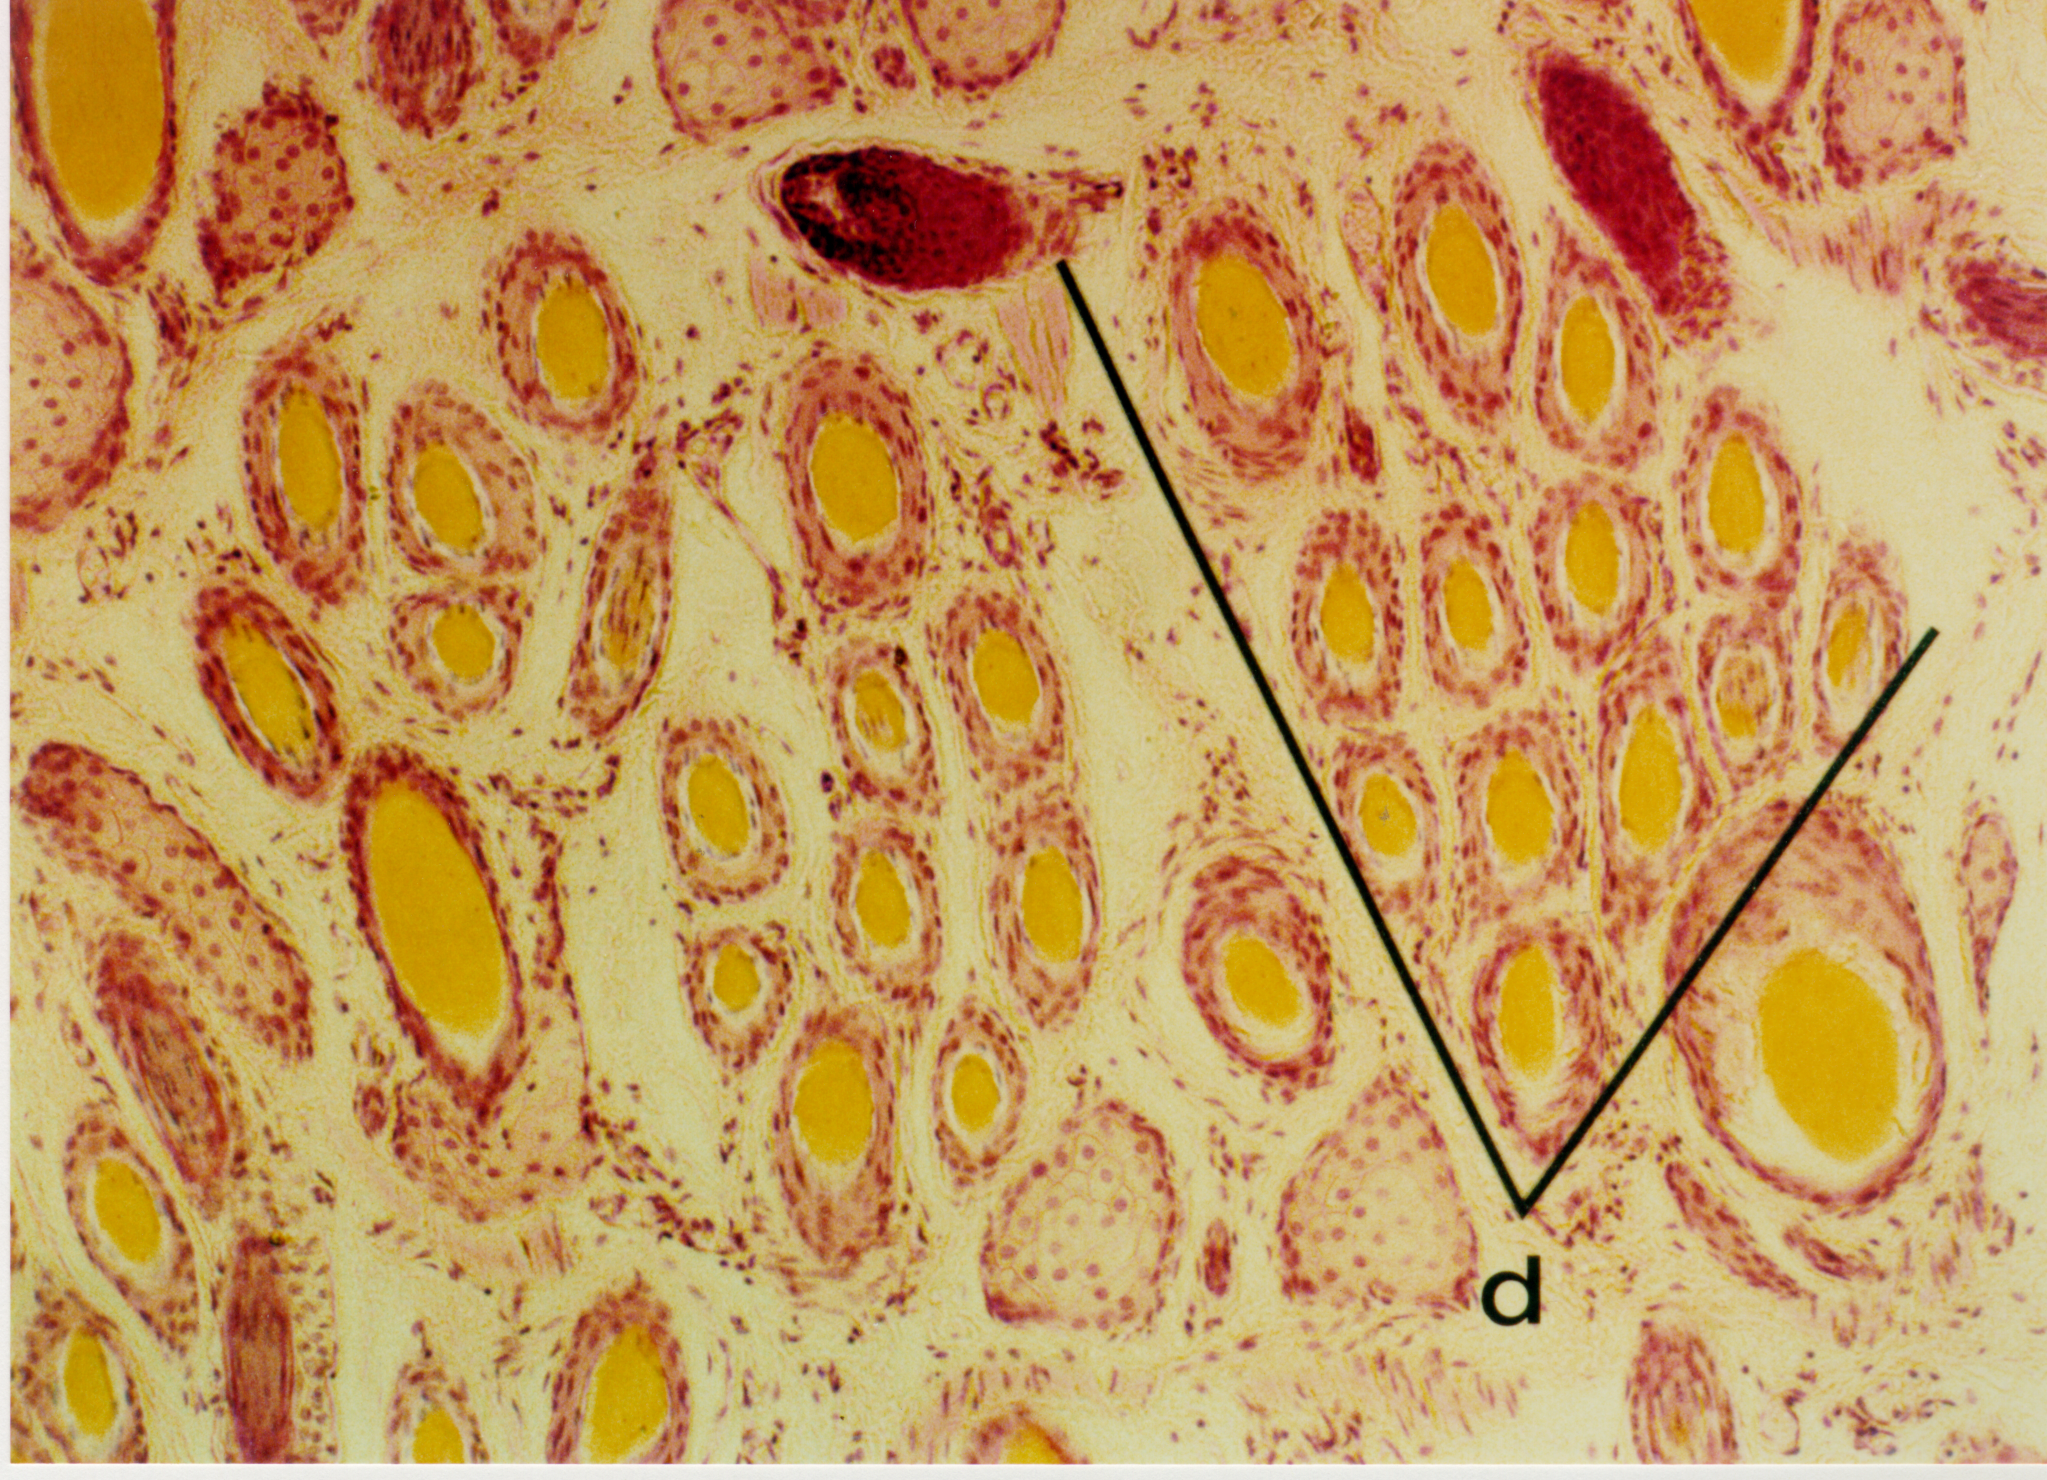
\includegraphics[width=0.65\textwidth, trim = 0 20 0 20]{images/fig9c.png}
  }
      \caption{ Transverse section of skin from the Australian Merino specimen
      of Figure~\ref{fig:8}.  Note (a) central primary follicle from which fibre
      has shed, (b) large lateral primary fibres (40 $\mu m$), (c) central
      primary fibre with fine fibre regrowth tip (78 $\mu m$), (d) wedge shaped
      arrangement of secondary follicles extending between the row of primary
      follicles, similar to the ancient fine/medium wool in Figure~\ref{fig:7}.}
  \label{fig:9}
\end{figure}

%\end{landscape}
%\end{document}
